\documentclass[crop,tikz]{standalone}
\usepackage{tikz}
\usepackage{amsmath}

\usetikzlibrary{positioning}

\begin{document}
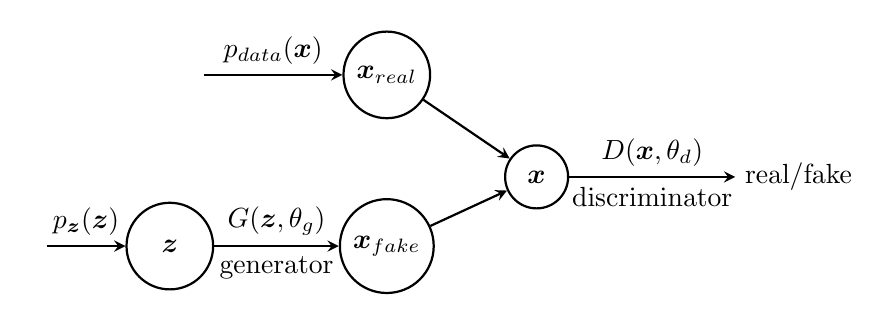
\begin{tikzpicture}

	\node[circle, draw, thick, minimum size=1.1cm] (z) {$\boldsymbol{z}$};
	\node[circle, draw, thick, right=4.5em of z, minimum size=1.1cm] (x) {$\boldsymbol{x}_{fake}$};
	\draw[-stealth, thick] (z) -- node[above] {$G(\boldsymbol{z},\theta_{g})$} node[below] {generator} (x);
	\node[left=of z] (i) {};
	\draw[-stealth, thick] (i) -- node[above] {$p_{\boldsymbol{z}}(\boldsymbol{z})$} (z);
	\node[above=of x, circle, draw, thick,minimum size=1.1cm] (xt) {$\boldsymbol{x}_{real}$};
	\node[left=5em of xt] (it) {};
	\draw[-stealth, thick] (it) -- node[above] {$p_{data}(\boldsymbol{x})$} (xt);
	\node[circle, draw, thick, right=2.5em of x, yshift=2.5em, minimum size=0.8cm] (D) {$\boldsymbol{x}$};
	\node[right=6em of D] (out) {real/fake};
	\draw[-stealth, thick] (D) -- node[above] {$D(\boldsymbol{x},\theta_{d})$} node[below] {discriminator} (out);

	
	\draw[-stealth, thick] (xt) -- (D);
	\draw[-stealth, thick] (x) -- (D);

\end{tikzpicture}
\end{document}